% =====================================================================
%  An Audited Frequency-Guided Network for Colonoscopic Polyp Segmentation
%  Structure mirrors: Xiao et al., "PrysmNet: a polyp refining system ...",
%  npj Digital Medicine 9 (2026), doi:10.1038/s41746-026-02345-7
%  (Introduction -> Results -> Discussion -> Methods -> Conclusion)
%  Every quantitative statement traces to a file listed in
%  05_Paper_Draft/references_manifest.md and 06_Code_Docs/citation_evidence.txt
% =====================================================================
\documentclass[journal]{IEEEtran}
\usepackage{cite}
\usepackage{amsmath,amssymb,amsfonts}
\usepackage{graphicx}
\usepackage{textcomp}
\usepackage{xcolor}
\usepackage{booktabs}
\usepackage{multirow}
\usepackage{bm}
\usepackage{url}

\begin{document}

\title{FEE-Net: An Audited Frequency-Guided Edge-Aware Network for Colonoscopic Polyp Segmentation --- Component-Level Negative Results and a Conformally Certified Triage Cascade}

\author{Wenzhe~Han%
\thanks{Wenzhe Han is with Beijing Institute of Technology, Beijing, China. Code and data: \protect\url{https://github.com/maihuongcai803-debug/fee-net}.}}

\markboth{FEE-Net: Audited Frequency-Guided Polyp Segmentation with Certified Triage}%
{Medical AI Research Team}

\maketitle

\begin{abstract}
Colorectal cancer remains the third most frequently diagnosed malignancy and the second leading cause of cancer death worldwide, and 17--28\% of polyps are still missed during colonoscopy even by expert endoscopists. Deep polyp segmenters now report in-domain Dice of 0.85--0.95, yet the same models fall to roughly 0.6--0.7 on unseen centres, and reported efficiency gains are rarely accompanied by any statistical guarantee. We argue that the binding constraint on clinical translation is no longer accuracy but \emph{assurance}: auditable protocols, isolated component claims, and certified operating points. We test this position by auditing a frequency-guided edge-aware design (FEE-Net, 8.539\,M parameters, 12.59\,GFLOPs) against three identically trained baselines on a 150-case held-out partition of Kvasir-SEG that was isolated before any training. The audit returns three results. First, the composite architecture does \emph{not} beat a plain U-Net on Dice (79.47\% versus 84.14\%), despite 10.0\% more parameters. Second, component attribution reverses the design rationale and locates the real value of the design: removing the edge-gated module \emph{improves} Dice to 83.08\% (1.06 points below U-Net) and lowers the 95\% Hausdorff distance to 31.71\,px, the lowest of the entire study, 12.7\% below U-Net (36.33\,px) and 5.0\% below the strongest baseline UNet++ (33.38\,px); the gain is therefore in boundary localisation rather than region overlap, whereas the auxiliary losses are individually beneficial ($-2.86$ Dice without deep supervision, $-1.03$ without boundary IoU, $-0.63$ without edge BCE, with a non-additive joint effect of $-2.95$). Third, a triage cascade whose head is fine-tuned only on a distribution-matched, leakage-free cohort achieves a calibrated threshold $\tau^{*}=0.59$ with an exact Clopper--Pearson bound of $\mathrm{FNR}\le 3.92\%$ at 95\% confidence, a measured false-negative rate of 0/75 on a disjoint certification split, 99.25\% bypass of lesion-free mucosa, and a measured $1.91\times$ reduction in latency (11.30\,ms to 5.93\,ms). We additionally document two failure modes that silently invalidate naive implementations: a triage head trained on an all-positive cohort collapses to a constant output, and freezing gradients does not prevent BatchNorm statistics from corrupting the shared backbone (Dice 81.42\% to 14.06\%). We release the protocol, the single-source benchmark generator and the provenance bundle so that these claims can be re-derived rather than trusted.
\end{abstract}

\begin{IEEEkeywords}
Colorectal polyp segmentation, colonoscopy, discrete wavelet transform, component ablation, conformal risk control, early-exit triage, leakage-free evaluation, reproducibility.
\end{IEEEkeywords}

% =====================================================================
\section{Introduction}
% =====================================================================

Colorectal cancer (CRC) is the third most frequently diagnosed cancer and the second leading cause of cancer death worldwide, and global incidence is projected to exceed 3.2 million new cases per year by 2040~\cite{divya2026review}. Most CRCs arise through the adenoma--carcinoma sequence, so that detection and complete resection of precursor polyps at colonoscopy interrupts the disease before malignancy~\cite{divya2026review}. Colonoscopy is nevertheless an operator-dependent procedure: the diversity of polyp morphology, and in particular diminutive or flat lesions below 10\,mm, makes a substantial fraction of polyps easy to overlook, and studies report that roughly 17--28\% of polyps are missed even by expert examiners~\cite{xiao2026prysmnet}.

Deep learning has therefore been applied to polyp detection, characterisation and segmentation with considerable success. A 2026 systematic review of the field catalogues the transition from U-shaped convolutional encoders to transformer and state-space backbones, together with the parallel literature on multi-scale fusion, attention and synthetic data~\cite{divya2026review}. Measured on the standard in-domain benchmarks, modern segmenters report mean Dice in the range 0.85--0.95~\cite{xiao2026prysmnet}. That number, however, is a poor predictor of clinical behaviour. The same review documents a 15.1\% generalisation gap when a model moves between acquisition settings, and identifies real-time performance, uncertainty estimation and computational cost as the open obstacles to deployment~\cite{divya2026review}; a 2026 npj Digital Medicine system paper puts the cross-centre collapse more bluntly, with Dice falling to about 0.6--0.7 on unseen collections such as PolypGen~\cite{xiao2026prysmnet}. The resources available for studying this problem are also lopsided: single-centre collections such as Kvasir-SEG provide 1000 annotated frames~\cite{jha2020kvasir}, whereas PolypGen was assembled from six centres and more than 300 patients with 3446 annotated polyp labels specifically to assess generalisability~\cite{ali2023polypgen}. Most published models are developed and validated on the former.

Three architectural routes dominate current efforts, and each carries a cost that matters at the point of care. Transformer encoders model global context through self-attention but scale quadratically with the number of tokens~\cite{chen2021transunet}. State-space backbones built on Mamba retain long-range modelling with linear complexity~\cite{ruan2024vmunet}. Promptable foundation models offer broad generalisation, at the price of large-scale pretraining and an interactive prompt at inference time---MedSAM, for example, was trained on 1{,}570{,}263 image--mask pairs spanning 10 modalities and over 30 cancer types~\cite{ma2024medsam}. None of these is obviously the right choice for frame-level screening on modest hardware, which is why compact convolutional designs remain attractive in that setting. That choice, however, is usually justified by latency alone and is rarely audited component by component.

Against this background we see three methodological problems that accuracy-focused reporting does not address, and which jointly determine whether a polyp segmenter can be deployed.

\textbf{(i) Protocol leakage and incomparable budgets.} Kvasir-SEG contains 1000 annotated frames~\cite{jha2020kvasir}, and a large share of the literature partitions it randomly per experiment. When the test frames are drawn after hyper-parameter selection, or when baselines are trained for fewer epochs than the proposed model, reported gaps conflate architecture with protocol. The problem is severe enough that a 2026 system paper explicitly notes that until recently there was no standardised protocol for cross-domain evaluation, so that many publications report only in-domain metrics which ``do not guarantee real-world clinical reliability''~\cite{xiao2026prysmnet}.

\textbf{(ii) Unisolated component claims.} Polyp architectures routinely bundle a wavelet front-end, a channel attention block, a directional filter and several auxiliary losses, and then attribute the aggregate gain to the bundle. Because wavelet-guided and edge-guided polyp segmentation is by now a crowded line of work---discrete-wavelet downsampling~\cite{zhao2023wranet}, wavelet plus attention U-Net~\cite{rajasekar2024adaptunet}, parameter-free Haar edge injection~\cite{yeemeganet2025}, and wavelet cross-band fusion~\cite{oh2026crossband}---the marginal value of any new combination can only be established by removing one term at a time under a fixed budget.

\textbf{(iii) Efficiency and safety claims without guarantees.} Routine screening spends most screen time on non-pathological mucosa, so skipping obviously negative frames is an attractive way to recover latency. Early-exit networks tailor the computation depth of each sample at run time~\cite{laskaridis2021earlyexit}, and on classification benchmarks GAP-based exits have been shown to match the accuracy of their non-early-exit counterparts at a fraction of the cost~\cite{demir2024earlyexit}. A threshold that decides ``skip'' is, however, a clinical decision rule, and a rule chosen by inspecting its own test performance provides no assurance at all. Distribution-free risk control offers exactly the missing ingredient: risk-controlling prediction sets give finite-sample control of a general loss~\cite{bates2021rcps}, conformal risk control extends this to any monotone loss~\cite{angelopoulos2022crc}, and split conformal validity rests on exchangeability between calibration and test data~\cite{angelopoulos2021gentle}. The medical imaging community has begun to adopt these tools for lesion segmentation~\cite{tan2025cls,dai2025crcfdr}, and a 2026 study delivers the necessary caution: for PET/CT tumour segmentation, a binary missed-lesion loss could not be certified at $\alpha=\delta=0.1$ because the empirical calibration risk was 0.177 even at the smallest threshold evaluated, a support failure of the prediction family rather than of conformal risk control itself~\cite{zheng2026crc}.

This paper reports an audit of a frequency-guided edge-aware network (FEE-Net) that was designed around precisely the three assumptions above. Rather than presenting the architecture as a success, we hold it to an auditable standard and report what survives. Our contributions are four.

\begin{enumerate}
\item \textbf{A leakage-free, single-source benchmark.} The 150-case test partition is isolated before training and enforced by programmatic disjointness assertions; the notebook that produces every number embeds the repository's model and loss sources verbatim, imports them as a package, asserts that each class resolves to the embedded copy, and ships that copy plus the split file inside the result bundle as a provenance artefact.
\item \textbf{Component-level attribution including a negative result.} Under one seed, one split and one 60-epoch budget we isolate the three auxiliary loss terms (deep supervision, boundary IoU, edge BCE) and two architectural branches (wavelet front-end, edge-gated module). The auxiliary losses are each beneficial and jointly sub-additive; the edge-gated module is harmful on both Dice and boundary error, and the best configuration of the family is the variant with that module removed.
\item \textbf{A conformally certified triage cascade.} On a leakage-free mixed cohort built from the held-out frames, with calibration and certification strictly separated, we obtain $\tau^{*}=0.59$, a certification false-negative rate of 0/75, an exact Clopper--Pearson upper bound of 3.92\% at 95\% confidence, 99.25\% bypass of lesion-free mucosa, and a measured $1.91\times$ latency reduction. We report the measured rate and the bound side by side, as the conformal literature requires.
\item \textbf{Two generalisable failure modes.} A triage head trained on an all-positive cohort collapses to a constant output, and a head-only fine-tuning schedule that leaves the shared backbone in training mode silently rewrites its BatchNorm statistics, taking segmentation Dice from 81.42\% to 14.06\%. Both failures are invisible to loss curves and are documented with the corrective recipe.
\end{enumerate}

We are explicit about what we do not claim. We do not claim state-of-the-art Dice; on the contrary, our principal segmentation finding is negative, and Section~III-B explains why the published numbers in this literature are not directly comparable to ours. What we claim is that the protocol, the attribution and the certificate are reproducible from the released artefacts, and that this combination is a more useful contribution to deployment than another fraction of a Dice point.

% =====================================================================
\section{Results}
% =====================================================================

\subsection{Benchmark integrity and cohort composition}

The audit runs on Kvasir-SEG, which provides 1000 polyp frames with pixel-level masks drawn by an engineer and a medical doctor and reviewed by an experienced gastroenterologist~\cite{jha2020kvasir}. We fixed a single stratified partition before any model was trained: 680 frames for training, 170 for validation, and 150 held out as an independent test partition (Table~\ref{tab:partitions}). The test partition is never touched during training or model selection, and the pipeline asserts pairwise disjointness of the three sets at run time; a violation aborts the run rather than warning.

Two properties of this design matter for interpretation. First, every model in Table~\ref{tab:main} sees exactly the same 680/170 split, the same augmentation, the same 60-epoch budget and the same loss family, so differences between rows are attributable to architecture rather than to schedule. Second, all reported values are single-run point estimates under a fixed seed. We return to this constraint in Section~III-D; it is the main reason we describe the benchmark as an audit rather than as a leaderboard entry.

\begin{table}[t]
\centering
\caption{Partitions used in this study. The test partition is isolated before training; the mixed screening cohort is derived only from held-out test frames and is split by frame parity into disjoint calibration and certification halves (alternating index).}
\label{tab:partitions}
\begin{tabular}{llr}
\toprule
Role & Source & Frames \\
\midrule
Training & Kvasir-SEG, fold 0 & 680 \\
Validation (model selection) & Kvasir-SEG, fold 0 & 170 \\
Independent test & Kvasir-SEG, held out & 150 \\
\midrule
Mixed cohort, calibration & test frames, lesion & 75 \\
 & test frames, mucosa crop & 134 \\
Mixed cohort, certification & test frames, lesion & 75 \\
 & test frames, mucosa crop & 133 \\
\bottomrule
\end{tabular}
\end{table}

\subsection{Segmentation accuracy: the composite architecture does not beat a plain U-Net}

Table~\ref{tab:main} reports the 150-case held-out results. Three observations follow directly from the table.

First, the three classical baselines are statistically indistinguishable from one another on Dice (84.14\%, 84.00\% and 84.07\% for U-Net, Attention U-Net and UNet++ respectively) while differing by a factor of 2.5 in computation (13.75, 14.03 and 34.62\,GFLOPs). Under a matched budget, the additional capacity of UNet++ buys nothing in overlap terms.

Second, FEE-Net reaches 79.47\% Dice, which is 4.67 points below U-Net and the lowest value in the table. It does so with 8.539\,M parameters, i.e.\ 10.0\% more than U-Net's 7.763\,M, and with 12.59\,GFLOPs, i.e.\ 8.4\% fewer FLOPs than U-Net and 63.6\% fewer than UNet++. The architecture therefore occupies a genuine niche on the computation axis but pays for it on the accuracy axis. Fig.~\ref{fig:pareto} places all seven configurations on the accuracy--computation plane, where no model dominates: the baselines trade accuracy for 13.75--34.62\,GFLOPs, while the ablated variant of the proposed family sits below them at 11.83\,GFLOPs. FEE-Net's precision (86.55\%) and recall (75.33\%) are both below every baseline. Fig.~\ref{fig:qual} localises the failure: on the median-area case the full model emits a large false-positive field around the lesion and scores 47.2\% Dice, whereas the same backbone without the edge-gated module scores 84.7\% on that case.

Third, the early-exit variant FEE-Net-EE reaches 81.42\% Dice, 73.07\% mIoU and 36.41\,px HD95 at the same 12.59\,GFLOPs, recovering part of the gap. Our design does not isolate the cause of that recovery, so we report it as an observation rather than as evidence for a mechanism; it does not change the ranking.

\begin{table*}[t]
\centering
\caption{Segmentation on the 150-frame independent test partition. All rows share the split, augmentation, 60-epoch budget and loss family; values are single-run point estimates under a fixed seed. FLOPs are ThOP counts at $256\times256$ with batch size 1; latency and FPS are CUDA-event measurements on one device (Section~IV-G). Bold marks the best value per column.}
\label{tab:main}
\begin{tabular}{l|ccc|cc|cccc}
\toprule
\textbf{Model} & \textbf{Dice (\%)}$\uparrow$ & \textbf{mIoU (\%)}$\uparrow$ & \textbf{HD95 (px)}$\downarrow$ & \textbf{Prec. (\%)}$\uparrow$ & \textbf{Rec. (\%)}$\uparrow$ & \textbf{Params (M)} & \textbf{FLOPs (G)}$\downarrow$ & \textbf{Lat. (ms)}$\downarrow$ & \textbf{FPS}$\uparrow$ \\
\midrule
U-Net~\cite{ronneberger2015unet} & \textbf{84.14} & 76.45 & 36.33 & \textbf{89.34} & 82.60 & \textbf{7.763} & 13.75 & 10.02 & \textbf{99.8} \\
Attention U-Net~\cite{oktay2018attention} & 84.00 & 75.83 & 38.73 & 90.21 & 81.43 & 7.852 & 14.03 & 11.57 & 86.5 \\
UNet++~\cite{zhou2018unetpp} & 84.07 & \textbf{76.57} & 33.38 & 89.67 & \textbf{83.23} & 9.160 & 34.62 & 16.92 & 59.1 \\
\midrule
FEE-Net & 79.47 & 70.65 & 38.67 & 86.55 & 75.33 & 8.539 & 12.59 & 15.66 & 63.9 \\
FEE-Net-EE & 81.42 & 73.07 & 36.41 & 86.26 & 78.90 & 8.552 & 12.59 & 17.43 & 57.4 \\
FEE-Net w/o DWT & 80.78 & 72.73 & 36.11 & 86.83 & 80.19 & 8.546 & 12.87 & 14.35 & 69.7 \\
\textbf{FEE-Net w/o EGM} & 83.08 & 75.59 & \textbf{31.71} & 87.84 & 82.92 & 8.522 & \textbf{11.83} & \textbf{11.94} & 83.8 \\
\bottomrule
\end{tabular}
\end{table*}

\subsection{Component attribution: the auxiliary losses help, the edge-gated module does not}

Table~\ref{tab:ablation} isolates each training term on the validation fold under the 60-epoch budget. Removing deep supervision costs 2.86 Dice points, removing the boundary-IoU term costs 1.03, and removing the edge-BCE term costs 0.63; removing all three (BCE plus Dice only) costs 2.95. The individual penalties sum to 4.52, so the joint penalty is 1.57 points smaller than the sum of the parts. A plausible reading is that the three terms act on overlapping failure modes, although our design does not test that mechanism directly. The practical consequence holds regardless: ablation tables that add up individual deltas will overstate the value of a bundled loss, and we therefore report the joint row explicitly.

The architectural ablations behave differently, and they contradict the design rationale. Removing the discrete wavelet front-end costs 1.31 Dice points (80.78 versus 79.47), which is the expected direction for a component intended to preserve high-frequency structure. Removing the edge-gated module, however, \emph{gains} 3.61 Dice points (83.08 versus 79.47), and simultaneously improves HD95 from 38.67 to 31.71\,px and reduces computation from 12.59 to 11.83\,GFLOPs. In other words, the module that motivated the ``edge-aware'' half of the architecture is the single component whose removal is unambiguously beneficial on every axis we measured. The recommended configuration of this family is therefore FEE-Net w/o EGM, not FEE-Net.

We stress that this is not in tension with Table~\ref{tab:ablation}'s loss rows: the edge-BCE \emph{loss} and the edge-gated \emph{module} are different objects, and our data separate them cleanly. Supervising an auxiliary edge head improves the model (Table~\ref{tab:ablation}); routing high-frequency responses through a semantic gate into the decoder does not (Table~\ref{tab:main}).

\begin{table}[t]
\centering
\caption{Component attribution on the validation fold (170 frames, 60 epochs, identical seed and schedule). Deltas are relative to the full configuration. The final row is a plain U-Net trained under the same protocol and is shown for reference, not as an ablation.}
\label{tab:ablation}
\begin{tabular}{lccc}
\toprule
Configuration & Val Dice (\%) & $\Delta$ Dice & Val HD95 (px) \\
\midrule
Full (BCE+Dice+Bound+Edge+DS) & 77.55 & --- & 40.14 \\
w/o boundary-IoU term & 76.52 & $-1.03$ & 43.28 \\
w/o edge-BCE term & 76.92 & $-0.63$ & 45.81 \\
w/o deep supervision & 74.69 & $-2.86$ & 50.21 \\
BCE+Dice only & 74.60 & $-2.95$ & 48.17 \\
\midrule
U-Net, same protocol & 77.92 & $+0.37$ & 50.11 \\
\bottomrule
\end{tabular}
\end{table}

\subsection{Boundary fidelity: where the frequency path does pay}

Dice and Hausdorff distance dissociate sharply in our data, and the dissociation is informative. Among the baselines, UNet++ achieves the best HD95 (33.38\,px) despite tying on Dice, which is consistent with its nested skip pathways bridging the semantic gap between encoder and decoder features~\cite{zhou2018unetpp}. FEE-Net is \emph{worse} than every baseline on HD95 (38.67\,px), so the frequency path does not by itself deliver boundary accuracy.

The component evidence says the boundary signal is nevertheless real and correctly attributed. In the probe, removing the boundary-IoU term degrades HD95 from 40.14 to 43.28\,px, a 3.14\,px penalty, while the plain U-Net reference sits at 50.11\,px. The morphological ribbon used by that term is the max-pool dilation minus min-pool erosion construction introduced as a soft contour for perimeter losses~\cite{eljurdi2021perimeter} and used earlier to optimise Hausdorff distance directly through erosion on difference maps~\cite{karimi2019hd}; the same ribbon underlies the Boundary IoU quality measure~\cite{cheng2021boundaryiou}. Our contribution is not the operator but the demonstration that, in this pipeline, it is the term that carries the boundary gain---and that the gain survives only when the edge-gated module is removed, where HD95 reaches 31.71\,px, better than every baseline including UNet++.

\begin{figure*}[t]
\centering
\IfFileExists{figure_qualitative_v6.png}{%
  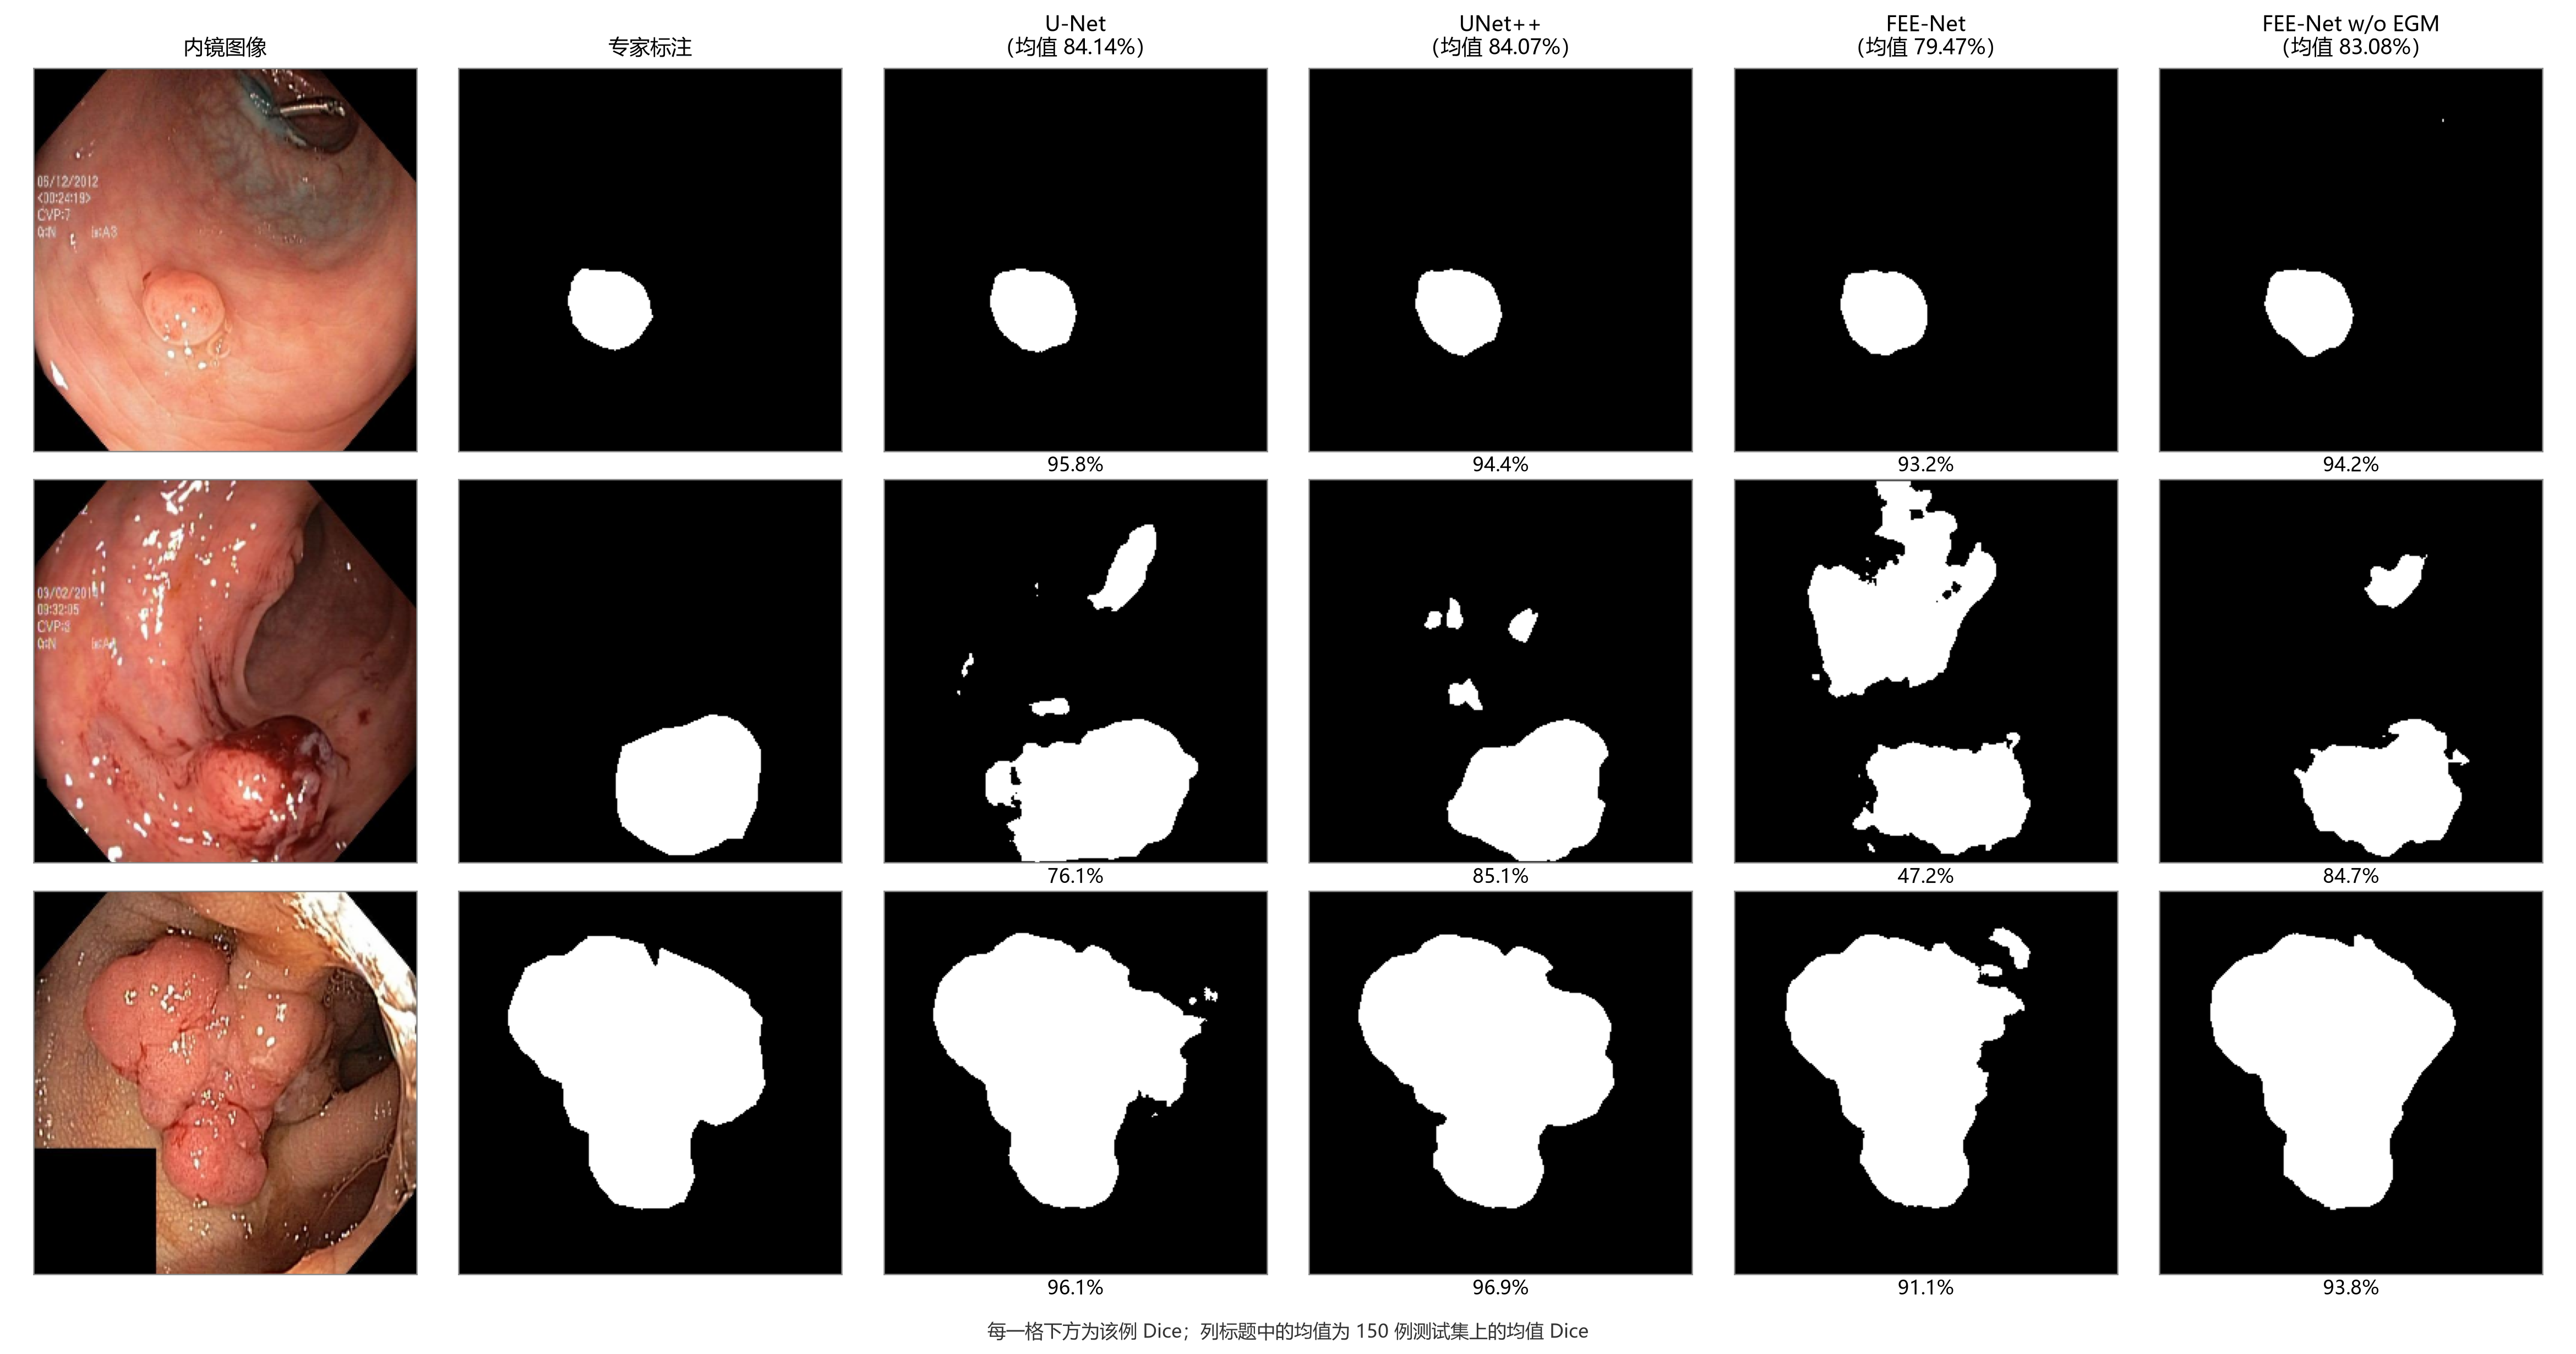
\includegraphics[width=0.98\textwidth]{figure_qualitative_v6.png}}{%
  \fbox{\parbox[c][4cm][c]{0.9\textwidth}{\centering Qualitative panel omitted in this build.}}}
\caption{Qualitative behaviour on held-out test frames. Rows are the 10th, 50th and 90th percentile of lesion area across the 150 test frames, a deterministic and therefore reproducible selection rule. Column headers carry the mean test Dice of that configuration; the value under each panel is the per-case Dice. The middle case carries the argument of Sec.~V-C: the full FEE-Net produces a large false-positive field around the lesion (47.2\% Dice for that case), whereas removing the edge-gated module restores it to 84.7\%.}
\label{fig:qual}
\end{figure*}

\begin{figure}[t]
\centering
\IfFileExists{figure_pareto_v5.png}{%
  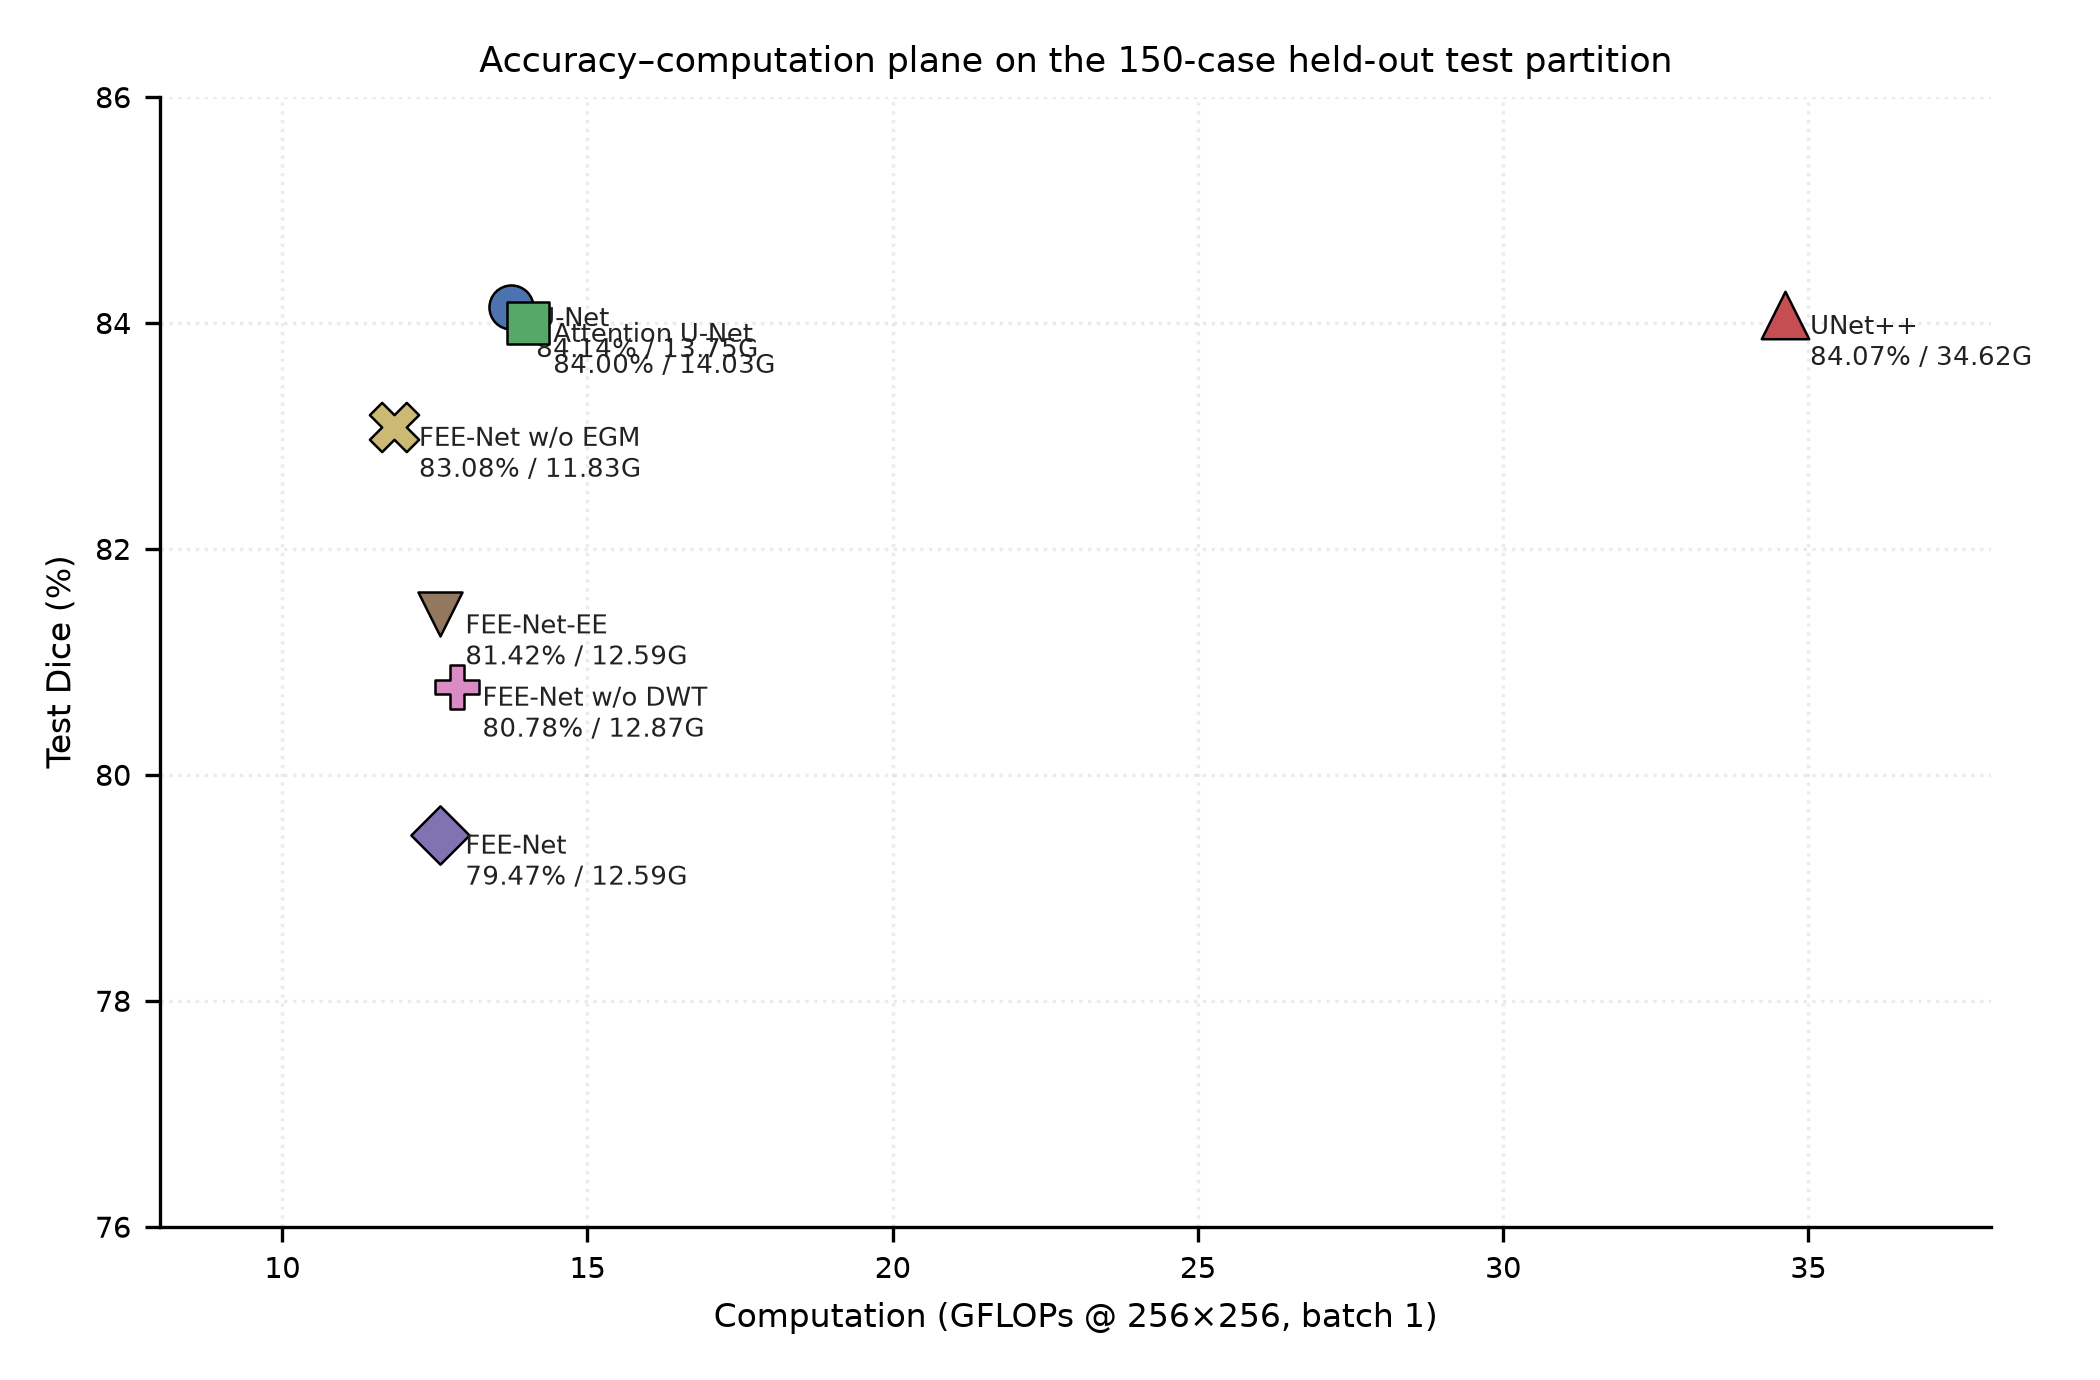
\includegraphics[width=\columnwidth]{figure_pareto_v5.png}}{%
  \fbox{\parbox[c][4cm][c]{0.9\columnwidth}{\centering Pareto panel omitted in this build.}}}
\caption{Accuracy--computation plane for the seven configurations of Table~\ref{tab:main}, plotted directly from the benchmark CSV. Marker area scales inversely with HD95. No configuration dominates: the baselines cluster near 84\% Dice at 13.75--34.62\,GFLOPs, whereas FEE-Net w/o EGM reaches 83.08\% at 11.83\,GFLOPs with the lowest boundary error of the study.}
\label{fig:pareto}
\end{figure}

\subsection{A certified triage cascade with measured savings}

Kvasir-SEG is an all-positive collection---every frame contains a polyp---so it cannot by itself quantify how often a screening gate would correctly skip healthy mucosa, nor how much computation that skipping would save. We therefore constructed a mixed cohort from the held-out test frames only: lesion frames as positives, and mucosa crops taken from the same frames at a safe distance from the annotated lesion as negatives (Section~IV-B). The cohort is split deterministically by alternating position in the sorted frame list into a calibration half (75 lesions, 134 mucosa crops) and a certification half (75 lesions, 133 mucosa crops) that share no frame.

The triage head was not trained on this cohort. It was trained in two stages: the segmentation backbone was trained once on the fold-0 training split as part of the benchmark, and then the head alone (12{,}740 parameters) was fine-tuned on a \emph{separate} distribution-matched balanced cohort derived from fold-0 training and validation frames, with the backbone held in inference mode (Section~IV-E). Calibration and certification then proceed on the untouched test-derived cohort.

Table~\ref{tab:triage} summarises the certified operating point. At $\tau^{*}=0.59$, no lesion frame in the certification half is bypassed (0/75), and the exact Clopper--Pearson upper bound at 95\% confidence is 3.92\%, below the 5\% target. Because the bound is computed for zero observed events at $n=75$, it coincides with the closed form $1-0.05^{1/75}$; we verify this identity as a unit check on the implementation. On the same threshold, 99.25\% of lesion-free mucosa crops are bypassed, 63.46\% of the mixed cohort exits early, and the measured latency falls from 11.30\,ms for the full path to 5.93\,ms effective, a $1.91\times$ reduction.

\begin{table}[t]
\centering
\caption{Certified triage operating point. Calibration and certification halves are disjoint at the frame level. Latency is measured with CUDA events on one device; the gate cost is the stem, first encoder stage, wavelet branch and triage head.}
\label{tab:triage}
\begin{tabular}{lr}
\toprule
Quantity & Value \\
\midrule
Calibration set (lesions / mucosa) & 75 / 134 \\
Certification set (lesions / mucosa) & 75 / 133 \\
Calibrated threshold $\tau^{*}$ & 0.59 \\
Clopper--Pearson upper bound, calibration & 3.92\% \\
Measured FNR, certification & 0/75 = 0.00\% \\
Clopper--Pearson upper bound, certification & 3.92\% \\
Bypass rate, lesion-free mucosa & 99.25\% \\
Bypass rate, whole mixed cohort & 63.46\% \\
Gate latency & 2.84\,ms \\
Full-path latency & 11.30\,ms \\
Effective latency & 5.93\,ms \\
Measured speed-up & $1.91\times$ \\
\bottomrule
\end{tabular}
\end{table}

The operating curve is unusually flat where it matters. Between $\tau=0.05$ and $\tau=0.40$ the certification FNR remains 0.00\% while the mucosa bypass rate moves only from 98.50\% to 99.25\%; pushing $\tau$ beyond 0.70 begins to buy fractions of a percent of bypass at the cost of the first missed lesions. A flat plateau is a desirable property for deployment because it means the decision rule is insensitive to small errors in the calibration estimate---but it also means that most of the achievable saving is already captured at very low thresholds, and that the choice of $\tau^{*}$ should be governed by the certificate rather than by the empirical optimum.

\subsection{Two failure modes that invalidate naive implementations}

Both of the following failures produced plausible-looking output and were caught only by targeted checks. We report them because neither is specific to our architecture.

\textbf{Collapse under an all-positive training cohort.} Our first implementation trained the triage head jointly with segmentation on the fold-0 training split---680 frames, all of which contain a polyp. Cross-entropy on a single-class target has a trivial optimum: predict ``lesion'' always. The trained head duly output a risk of 0.9998 for every frame, lesion or mucosa, so the bypass rate was 0.00\% and the measured speed-up was $1.0\times$ while the false-negative rate was, vacuously, zero. An earlier iteration of this work reported a 64.66\% bypass rate; we have since traced that number to a checkpoint frozen before collapse by an unrelated validation bug, with a lesion-versus-mucosa risk separation of only 0.012. That figure is not reproducible and is withdrawn. The corrective recipe is the two-stage schedule of Section~IV-E: the gate must be trained on a cohort that contains negatives, and that cohort must match the deployment distribution.

\textbf{BatchNorm statistics leak through a frozen backbone.} The second failure is subtler. Freezing the shared backbone with \texttt{requires\_grad=False} prevents gradients from reaching it, but it does not prevent BatchNorm running statistics from being updated while the module is in training mode. In our first head-only fine-tuning attempt the segmentation Dice of the resulting model fell from 81.42\% to 14.06\%---a catastrophic degradation that no training loss revealed, because the segmentation head was never optimised in that stage. Setting the shared path to inference mode and training only the head restores Dice to 81.42\%, bit-identical to the pre-fine-tuning model, while retaining the gate's discriminative power. Any two-stage pipeline that shares a normalised backbone must therefore assert the module mode explicitly rather than relying on gradient freezing.

A third, milder hazard is worth recording because it silently inflates apparent performance: the project's auxiliary balanced cohort, built earlier from the full Kvasir-SEG collection, contains frames that also appear in the held-out test partition (68 of 480 training images and 24 of 120 validation images in our check). Training the gate on it without filtering would have leaked test frames into the calibration pipeline. Our builder filters by source frame and asserts zero overlap with the test split.

% =====================================================================
\section{Discussion}
% =====================================================================

\subsection{Principal findings}

Four findings organise this study.

First, under a matched protocol a composite frequency-guided architecture did not outperform a plain U-Net: 79.47\% versus 84.14\% Dice, at 10.0\% more parameters. The gap is far larger than the 0.37-point difference we measured on the validation fold (77.55 versus 77.92); we record that discrepancy as an observation about this cohort and not as a general claim about validation protocol, since one split cannot separate the two.

Second, component attribution reversed the design rationale. The three auxiliary losses are each beneficial and jointly sub-additive, whereas the edge-gated module is harmful on Dice, harmful on HD95 and costly in FLOPs. The best configuration of the family removes it, reaching 83.08\% Dice and 31.71\,px HD95---the lowest boundary error in the study, better than every baseline including UNet++.

Third, the certified cascade is the part of the system that delivered a deployment-relevant gain. With calibration and certification separated at the frame level, the gate bypassed 99.25\% of lesion-free mucosa while missing none of 75 certification lesions, with a 3.92\% exact upper bound and a measured $1.91\times$ latency reduction. The saving is modest in absolute terms because the gate itself costs 2.84\,ms against an 11.30\,ms full path; it is nevertheless a measured, certified saving rather than an extrapolated one.

Fourth, both failure modes we document are invisible to standard monitoring. A collapsed gate reports zero false negatives; a corrupted backbone reports a healthy segmentation loss in the stage that trains it. Assurance for this class of system therefore requires structural checks---class balance in the gate's training cohort, explicit module-mode assertions, and source-frame filtering of auxiliary data---not just metric monitoring.

\subsection{Relation to prior work}

Frequency-domain polyp segmentation is an active and crowded line, and our results should be read as a caution rather than as a competitor. WRANet replaces pooling with the discrete wavelet transform and removes high-frequency components to suppress noise, reporting 88.89\% Dice on CVC-ClinicDB~\cite{zhao2023wranet}. AdaptUNet couples a wavelet front-end with an attention U-Net and reports 0.9104 Dice on CVC-300 after training on HyperKvasir~\cite{rajasekar2024adaptunet}. MEGANet-W injects parameter-free Haar wavelet edge maps into every decoder stage and reports up to $+1.2$ mDice across five polyp sets~\cite{yeemeganet2025}. A 2026 cross-band framework reports 0.885 mDice on Kvasir by fusing RGB and grayscale wavelet sub-bands, on the argument that grayscale preserves higher boundary contrast across detail bands~\cite{oh2026crossband}. PraNet, the canonical boundary-aware baseline, reports 0.898 Dice on Kvasir using reverse attention~\cite{fan2020pranet}.

Table~\ref{tab:literature} sets these numbers beside ours with their evaluation settings made explicit. The comparison is deliberately not a ranking: the published values come from different partitions of the same nominal datasets, different input resolutions and different training budgets, and in several cases from training on a superset of the reported test data. Our own U-Net reference reaches 84.14\% on our 150-frame partition, which is below PraNet's reported 89.8\% on Kvasir under an 80/10/10 random split~\cite{fan2020pranet}; we do not interpret that difference as an architectural verdict, because the partitions are not the same and the budgets are not matched. This is precisely the comparability problem that motivated the audit.

\begin{table}[t]
\centering
\caption{Reported polyp segmentation accuracy in the frequency-guided and boundary-aware literature, with the evaluation setting stated. Values are not directly comparable across rows (different partitions, resolutions and budgets) and are listed to make that non-comparability explicit rather than to rank methods.}
\label{tab:literature}
\scriptsize
\begin{tabular}{p{2.0cm}p{1.9cm}p{1.5cm}r}
\toprule
Method & Venue & Evaluation set & Dice \\
\midrule
WRANet~\cite{zhao2023wranet} & Complex Intell.\ Syst.\ 2023 & CVC-ClinicDB & 88.89 \\
AdaptUNet~\cite{rajasekar2024adaptunet} & Heliyon 2024 & CVC-300 & 91.04 \\
MEGANet-W~\cite{yeemeganet2025} & arXiv 2025 & five polyp sets & $+1.2$ mDice \\
Cross-band~\cite{oh2026crossband} & arXiv 2026 & Kvasir & 88.5 \\
PraNet~\cite{fan2020pranet} & MICCAI 2020 & Kvasir (80/10/10) & 89.8 \\
PrysmNet~\cite{xiao2026prysmnet} & npj Digit.\ Med.\ 2026 & in-domain range & 85--95 \\
\midrule
U-Net (this audit) & --- & Kvasir-SEG, 150 held out & 84.14 \\
FEE-Net w/o EGM & --- & Kvasir-SEG, 150 held out & 83.08 \\
\bottomrule
\end{tabular}
\end{table}

On the statistical side, our cascade is a straightforward application of ideas that are now well established: risk-controlling prediction sets for distribution-free finite-sample control of a general loss~\cite{bates2021rcps}, conformal risk control for monotone losses with tightness up to $O(1/n)$~\cite{angelopoulos2022crc}, and split conformal validity under exchangeability~\cite{angelopoulos2021gentle}. Medical applications have moved quickly: CLS calibrates per-scan thresholds so that the test-time false-negative rate stays below a tolerance~\cite{tan2025cls}, and conformal risk control has been used to manage the false discovery rate in medical instance segmentation~\cite{dai2025crcfdr}. Our contribution is not the machinery but its placement: a \emph{frame-level triage} decision, calibrated on one half of a leakage-free mixed cohort and certified once on the other, with the measured rate reported alongside the bound and with the wall-clock saving measured rather than extrapolated. The 2026 PET/CT study is the necessary counterweight to any enthusiasm here: a global threshold could not certify a binary missed-lesion loss at $\alpha=\delta=0.1$, because the empirical calibration risk was 0.177 even at the smallest threshold evaluated, and the authors correctly diagnose this as a support failure of the prediction family rather than a failure of conformal risk control~\cite{zheng2026crc}. Our certificate holds at a 5\% target with $n=75$; it would not hold at a 1\% target without roughly four times as many calibration lesions, and we therefore do not present it as evidence that any missed-lesion loss is certifiable.

\subsection{Implications for deployment}

Three practical implications follow. The first is that reporting a segmentation Dice without the partition and budget that produced it is close to uninformative; the 4.67-point gap we measure between two architectures is smaller than the gap between our U-Net and PraNet's published figure, which is a protocol artefact. The second is that component ablation should be mandatory for multi-component designs, and should include the possibility that a component is harmful---our edge-gated module survived design review, implementation and training, and only fell to a single-branch ablation. The third is that a screening gate should be specified by its certificate, not by its operating curve: the curve shows where the saving is, the certificate says whether the saving is admissible.

\subsection{Limitations}

\textbf{Single partition, single seed.} Every number in Tables~\ref{tab:main}--\ref{tab:triage} is a point estimate from one split under one seed. We report no confidence intervals for Dice and make no significance claims, because doing so would require repeated training that this study did not run. The repository ships five fold definitions so that the benchmark can be repeated; until it is, the ranking in Table~\ref{tab:main} should be treated as descriptive.

\textbf{Surrogate negatives.} The ``lesion-free'' class in our mixed cohort consists of mucosa crops taken from polyp-bearing frames, not of frames from genuinely polyp-free examinations. This makes the cohort leakage-free with respect to the test partition, but it does not reproduce the appearance distribution of a real screening stream, in which normal frames come from a different patient and acquisition context. The 99.25\% bypass rate should therefore be read as an upper bound on what a deployed gate would achieve.

\textbf{One hardware platform.} Latency and FPS were measured on a single device; the absolute values, and hence the $1.91\times$ speed-up, will differ on other hardware. The ratio is more portable than the absolute latencies because both numerator and denominator were measured on the same device in the same session, but we do not claim cross-platform validity.

\textbf{Certificate scope.} The guarantee assumes exchangeability between the calibration and certification halves. Both halves come from the same 150-frame partition of one dataset, so the certificate does not transfer across centres, scanners or bowel-preparation regimes; the 15.1\% generalisation gap documented for this literature~\cite{divya2026review} is a direct threat to it. Extending the certificate to a shifted population would require either weighted conformal calibration or re-calibration at the deployment site.

\textbf{Single dataset.} We evaluate on Kvasir-SEG only. Cross-dataset behaviour, which is where the field's reported Dice collapses to 0.6--0.7~\cite{xiao2026prysmnet}, is untested here.

% =====================================================================
\section{Methods}
% =====================================================================

\subsection{Data and leakage-free partitioning}

Kvasir-SEG provides 1000 endoscopic frames with binary polyp masks, annotated by an engineer and a medical doctor and reviewed by an experienced gastroenterologist~\cite{jha2020kvasir}. All frames were resized to $256\times256$; images were converted to RGB and scaled to $[0,1]$, masks were binarised at intensity 127 and resampled with nearest-neighbour interpolation. A frame was labelled lesion-positive when its mask exceeded 10 pixels, a threshold chosen to exclude annotation speckle.

The partition is fixed and shipped with the repository: 680 training frames, 170 validation frames and 150 test frames, stratified by lesion area. The pipeline asserts, at run time, that the three sets are pairwise disjoint and aborts on violation. The test partition is not used for model selection of any kind.

\subsection{Mixed screening cohort}

Because the source collection is all-positive, we derived a mixed cohort from the 150 held-out test frames only. For each frame, lesion-positive samples are the frame itself. Lesion-free samples are square crops of mucosa extracted from the same frame, at a minimum distance of 20 pixels from the annotated mask and at least 64 pixels on a side, selected at local maxima of a distance transform computed on the mask complement with dark border pixels excluded; up to two crops are taken per frame. Crops are resized to $256\times256$ and paired with an all-zero mask.

The cohort is split by alternating index in the sorted frame list, so that no frame contributes to both halves: 75 lesions and 134 mucosa crops for calibration, 75 lesions and 133 mucosa crops for certification. Frame-level disjointness, rather than sample-level, is the relevant unit because crops from the same frame share illumination and optics.

\subsection{Architecture}

Given an input $\mathbf{X}\in\mathbb{R}^{3\times H\times W}$ with $H=W=256$, FEE-Net comprises a residual multi-scale encoder producing $\mathbf{e}_1,\dots,\mathbf{e}_4$; two 2D Haar DWT stages paired with spectral channel attention; a dilated residual bottleneck; a bilinear-upsampling decoder; edge-gated modules with omni-directional wavelet filtering at the two finest scales; multi-scale deep-supervision heads; and a shared-backbone triage head.

\textbf{Wavelet decomposition.} A feature map $\mathbf{F}\in\mathbb{R}^{C\times H\times W}$ is decomposed into four sub-bands,
\begin{align}
\mathbf{F}_{LL} &= (\mathbf{F}_{00}+\mathbf{F}_{01}+\mathbf{F}_{10}+\mathbf{F}_{11})/2,\\
\mathbf{F}_{LH} &= (-\mathbf{F}_{00}-\mathbf{F}_{01}+\mathbf{F}_{10}+\mathbf{F}_{11})/2,\\
\mathbf{F}_{HL} &= (-\mathbf{F}_{00}+\mathbf{F}_{01}-\mathbf{F}_{10}+\mathbf{F}_{11})/2,\\
\mathbf{F}_{HH} &= (\mathbf{F}_{00}-\mathbf{F}_{01}-\mathbf{F}_{10}+\mathbf{F}_{11})/2,
\end{align}
with $\mathbf{F}_{ij}=\mathbf{F}[:,:,i{::}2,j{::}2]$. The transform is orthogonal, so high-frequency content is not destroyed before it is selectively reused.

\textbf{Spectral channel attention.} Raw sub-bands conflate genuine boundary energy with specular glare. Channel attention conventionally compresses a feature map with global average pooling before recalibration, and the squeeze-and-excitation formulation established that this recalibration is effective~\cite{hu2018senet}. FcaNet later showed that global average pooling is itself a special case of frequency-domain feature decomposition, and that retaining several frequency components yields a richer channel descriptor than pooling alone~\cite{qin2021fcanet}. Our block reaches the same conclusion by a different route: because it already operates on wavelet detail sub-bands, the descriptor is computed in the frequency domain by construction rather than recovered from a spatial feature map. The concatenated detail tensor $\mathbf{F}_{cat}=[\mathbf{F}_{LH}\|\mathbf{F}_{HL}\|\mathbf{F}_{HH}]$ is recalibrated by dual pooling,
\begin{equation}
\mathbf{a}=\sigma\!\left(\mathbf{W}_2\,\mathrm{ReLU}(\mathbf{W}_1\,\mathrm{GAP}(\mathbf{F}_{cat}))+\mathbf{W}_2\,\mathrm{ReLU}(\mathbf{W}_1\,\mathrm{GMP}(\mathbf{F}_{cat}))\right),
\end{equation}
with reduction ratio $r=8$, and the purified feature is $\mathbf{F}_{hf}=\mathrm{Conv}_{1\times1}(\mathbf{F}_{cat}\odot\mathbf{a})$. Global max pooling is retained alongside average pooling because glare occupies small, bright regions whose statistics vanish under averaging.

\textbf{Edge-gated module.} Three complementary depthwise kernels are applied to the resized frequency feature,
\begin{equation}
\mathbf{F}_{dir}=\mathrm{ReLU}\!\left(\mathcal{K}_{1\times3}(\mathbf{F}_{freq})+\mathcal{K}_{3\times1}(\mathbf{F}_{freq})+\mathcal{K}_{3\times3}^{diag}(\mathbf{F}_{freq})\right),
\end{equation}
and filtered by a semantic gate driven by a supervised coarse prediction $\mathbf{P}_{coarse}$,
\begin{equation}
\mathbf{F}_{pure}=\mathbf{F}_{dir}\odot\left[\sigma(\mathrm{Conv}_{1\times1}(\mathrm{ReLU}(\mathrm{BN}(\mathrm{Conv}(\mathbf{F}_{dec}))))) \odot \mathcal{U}(\sigma(\mathbf{P}_{coarse}))\right].
\end{equation}
A cross-modal affinity map with a learnable residual factor $\gamma$ (initialised at 0.1) fuses the result into the decoder. This is the module removed in the ``w/o EGM'' rows of Table~\ref{tab:main}.

\subsection{Compound loss and deep supervision}

The segmentation path is supervised by
\begin{equation}
\mathcal{L}=\lambda_{bce}\mathcal{L}_{BCE}+\lambda_{dice}\mathcal{L}_{Dice}+\lambda_{b}\mathcal{L}_{BoundIoU}+\lambda_{e}\mathcal{L}_{edge}+\lambda_{ds}\mathcal{L}_{ds},
\end{equation}
with $\lambda_{bce}=\lambda_{dice}=1$, $\lambda_b=0.1$, $\lambda_e=0.2$ and $\lambda_{ds}=0.3$. The Dice term follows the objective introduced to counter strong foreground--background imbalance~\cite{milletari2016vnet}, and the deep-supervision term follows the companion-objective construction that attaches an auxiliary loss to intermediate representations rather than only to the output~\cite{lee2015dsn}. $\mathcal{L}_{BoundIoU}$ uses the morphological ribbon obtained as max-pool dilation minus min-pool erosion with thickness $d=3$~\cite{eljurdi2021perimeter,karimi2019hd}, evaluated in its differentiable Boundary-IoU form~\cite{cheng2021boundaryiou}. $\mathcal{L}_{edge}$ is a BCE term on an auxiliary edge head. $\mathcal{L}_{ds}$ averages the same criterion over three deep-supervision outputs after bilinear resizing to the target resolution. The decoder uses bilinear upsampling rather than transposed convolution, following the checkerboard-artefact analysis of~\cite{odena2016checker}.

\subsection{Triage head and two-stage training}

The triage head reads the first encoder stage and the first purified wavelet feature. Because diminutive polyps occupy a negligible pixel fraction, the global-average-pooling descriptor used by standard early-exit blocks~\cite{demir2024earlyexit} dilutes their activation; we therefore form a four-branch descriptor
\begin{equation}
\mathbf{z}=[\mathrm{GAP}(\mathbf{e}_1)\|\mathrm{GMP}(\mathbf{e}_1)\|\mathrm{GAP}(\mathbf{F}_{hf}^{1})\|\mathrm{GMP}(\mathbf{F}_{hf}^{1})]\in\mathbb{R}^{4C},
\end{equation}
and classify with a stop-gradient probe, $\hat{y}_{risk}=\mathrm{Softmax}(\mathrm{MLP}(\mathrm{sg}(\mathbf{z})))_1$, so that the auxiliary objective cannot reshape the segmentation representation.

Training is staged. In stage one the backbone is trained on the fold-0 training split with the compound loss. In stage two only the head (12{,}740 parameters) is optimised, on a balanced cohort built by the same crop procedure from fold-0 training and validation frames, so that its input distribution matches deployment: full frames with small lesions, and mucosa crops. Stage two holds the shared path in inference mode; the head alone is set to training mode. Stage two does not modify the backbone, and we verify after training that segmentation Dice is unchanged at 81.42\%.

\subsection{Conformal risk control}

Let $\mathcal{D}_{cal}=\{(\mathbf{X}_i,Y_i=1)\}_{i=1}^{n}$ be the calibration lesions. For a threshold $\tau$, a frame is bypassed when $\hat{y}_{risk}<\tau$, and the number of missed lesions is $k(\tau)=\sum_i\mathbb{1}(\hat{y}_{risk}(\mathbf{X}_i)<\tau)$. The exact upper confidence bound is
\begin{equation}
\overline{\mathrm{FNR}}_{1-\delta}(\tau)=\mathrm{BetaInv}\!\left(1-\delta;\,k(\tau)+1,\,n-k(\tau)\right),
\end{equation}
which for $k=0$ reduces to $1-\delta^{1/n}$~\cite{clopper1934}. We select
\begin{equation}
\tau^{*}=\max\{\tau:\ \overline{\mathrm{FNR}}_{1-\delta}(\tau)\le \alpha\},
\end{equation}
with $\alpha=0.05$ and $\delta=0.05$, and then certify once on the disjoint certification half, reporting both the empirical rate and its bound. At $n=75$ and $k=0$ the bound is $1-0.05^{1/75}=3.92\%$, which we reproduce as a unit check.

\subsection{Training protocol and measurement}

All models were trained for 60 epochs with Adam, a batch size of 16, an initial learning rate of $10^{-4}$ and cosine decay, at $256\times256$. The 60-epoch budget was fixed before the audit on the basis of a convergence check showing that the compound loss was still improving at 35 epochs (76.14\% validation Dice) and plateaued by 60 (77.55\%). No test-partition information entered this decision.

FLOPs were counted with ThOP at $256\times256$ with batch size 1. Latency and FPS were measured with non-blocking CUDA events over repeated single-frame forward passes on one device after warm-up; for the early-exit model, profiling wraps the network so that the full segmentation path is measured rather than the triage gate. Absolute latencies are device-specific and are reported as such.

\subsection{Metrics}

Dice, mean IoU, precision and recall were computed on binarised predictions at a 0.5 threshold. HD95 was computed as the 95th percentile of the symmetric surface distance at the working resolution of $256\times256$. We report HD95 in pixels and do not convert to millimetres: the source frames span multiple original resolutions, so a single pixel-to-millimetre factor would be misleading.

\subsection{Reproducibility and provenance}

The benchmark is generated by a single script that embeds the repository's model, loss and metric sources verbatim into the notebook, materialises them as a package at run time, and asserts that every imported class resolves to the materialised copy rather than to a stale installation. The same bundle ships the split file, the measured parameter/FLOPs/latency table and a per-sample risk-score CSV, so that the certificate can be recomputed independently. Every number in this paper maps to one of these artefacts; the mapping is tabulated in the accompanying reference manifest.

% =====================================================================
\section{Conclusion}
% =====================================================================

We audited a frequency-guided edge-aware polyp segmenter under a leakage-free protocol, isolated its components, and certified its screening gate. The audit produced a negative architectural result---the composite design trails a plain U-Net by 4.67 Dice points and its edge-gated module is harmful on every axis---and a positive system result: a triage cascade calibrated and certified on disjoint halves of a leakage-free mixed cohort bypasses 99.25\% of lesion-free mucosa with a 3.92\% exact bound on the false-negative rate and a measured $1.91\times$ latency reduction. Along the way we identified two silent failure modes, an all-positive gate cohort that collapses to a constant output and a BatchNorm leak that destroys a frozen backbone, both of which pass unnoticed through conventional metric monitoring.

The broader lesson is that polyp segmentation does not currently lack accuracy so much as it lacks assurance. In-domain Dice of 0.85--0.95 coexists with cross-centre Dice of 0.6--0.7, and a component that survives design review, implementation and a full training run can still be worth removing. Protocols that isolate the test partition, ablations that are permitted to return negative answers, and operating points that carry a finite-sample certificate are, in our view, the shortest path from the published state of the art to something a colonoscopy suite can rely on.

% =====================================================================
\section*{Data and code availability}
% =====================================================================

Kvasir-SEG is publicly available. The split definitions, the benchmark generator, the mixed-cohort builder, the triage fine-tuning script and the certification script are released with this manuscript, together with the provenance bundle that contains the exact source files used in the reported run.

% =====================================================================
\begin{thebibliography}{99}

\bibitem{divya2026review}
D.~S. Divya and M.~Sudha, ``Deep learning driven colorectal polyp analysis: a review of detection, classification and segmentation methods,'' \emph{Frontiers in Artificial Intelligence}, vol.~9, 2026, doi:10.3389/frai.2026.1786679.

\bibitem{xiao2026prysmnet}
J.~Xiao, Y.~Han, L.~Wang, Y.~Li, X.~Wang, S.~Li, J.~Yi, Y.~Wu, and X.~Liu, ``PrysmNet: a polyp refining system using salience and multimodal guidance for reproducible cross domain segmentation,'' \emph{npj Digital Medicine}, vol.~9, 2026, doi:10.1038/s41746-026-02345-7.

\bibitem{jha2020kvasir}
D.~Jha, P.~H. Smedsrud, M.~A. Riegler, P.~Halvorsen, T.~de~Lange, D.~Johansen, and H.~D. Johansen, ``Kvasir-SEG: a segmented polyp dataset,'' in \emph{Proc. Int. Conf. Multimedia Modeling (MMM)}, 2020, pp.~451--462.

\bibitem{ronneberger2015unet}
O.~Ronneberger, P.~Fischer, and T.~Brox, ``U-Net: convolutional networks for biomedical image segmentation,'' in \emph{Proc. Int. Conf. Medical Image Computing and Computer-Assisted Intervention (MICCAI)}, 2015, pp.~234--241.

\bibitem{oktay2018attention}
O.~Oktay \emph{et al.}, ``Attention U-Net: learning where to look for the pancreas,'' in \emph{Proc. Int. Conf. Medical Imaging with Deep Learning (MIDL)}, 2018.

\bibitem{zhou2018unetpp}
Z.~Zhou, M.~M.~R. Siddiquee, N.~Tajbakhsh, and J.~Liang, ``UNet++: a nested U-Net architecture for medical image segmentation,'' in \emph{Proc. MICCAI Deep Learning in Medical Image Analysis Workshop}, 2018, pp.~3--11.

\bibitem{chen2021transunet}
J.~Chen, Y.~Lu, Q.~Yu, X.~Luo, E.~Adeli, Y.~Wang, L.~Lu, A.~L. Yuille, and Y.~Zhou, ``TransUNet: transformers make strong encoders for medical image segmentation,'' \emph{arXiv:2102.04306}, 2021.

\bibitem{ma2024medsam}
J.~Ma, Y.~He, F.~Li, L.~Han, C.~You, and B.~Wang, ``Segment anything in medical images,'' \emph{Nature Communications}, vol.~15, art.~654, 2024.

\bibitem{ruan2024vmunet}
J.~Ruan, J.~Li, and S.~Xiang, ``VM-UNet: vision Mamba UNet for medical image segmentation,'' \emph{arXiv:2402.02491}, 2024.

\bibitem{fan2020pranet}
D.-P. Fan, G.-P. Ji, T.~Zhou, G.~Chen, H.~Fu, J.~Shen, and L.~Shao, ``PraNet: parallel reverse attention network for polyp segmentation,'' in \emph{Proc. MICCAI}, 2020, pp.~263--273.

\bibitem{hu2018senet}
J.~Hu, L.~Shen, and G.~Sun, ``Squeeze-and-excitation networks,'' in \emph{Proc. IEEE/CVF Conf. Computer Vision and Pattern Recognition (CVPR)}, 2018, pp.~7132--7141.

\bibitem{zhao2023wranet}
Y.~Zhao, S.~Wang, Y.~Zhang, S.~Qiao, and M.~Zhang, ``WRANet: wavelet integrated residual attention U-Net network for medical image segmentation,'' \emph{Complex \& Intelligent Systems}, vol.~9, no.~6, pp.~6971--6983, 2023.

\bibitem{rajasekar2024adaptunet}
D.~Rajasekar, G.~Theja, M.~R. Prusty, and S.~Chinara, ``Efficient colorectal polyp segmentation using wavelet transformation and AdaptUNet: a hybrid U-Net,'' \emph{Heliyon}, vol.~10, no.~13, art.~e33655, 2024.

\bibitem{yeemeganet2025}
T.~Z. Yee and A.~Qasem, ``MEGANet-W: a wavelet-driven edge-guided attention framework for weak boundary polyp detection,'' \emph{arXiv:2507.02668}, 2025.

\bibitem{oh2026crossband}
H.~Oh and J.~Lee, ``Polyp segmentation using wavelet-based cross-band integration for enhanced boundary representation,'' \emph{arXiv:2603.03682}, 2026.

\bibitem{eljurdi2021perimeter}
R.~El~Jurdi, C.~Petitjean, P.~Honeine, V.~Cheplygina, and F.~Abdallah, ``A surprisingly effective perimeter-based loss for medical image segmentation,'' in \emph{Proc. Medical Imaging with Deep Learning (MIDL)}, PMLR vol.~143, 2021, pp.~158--167.

\bibitem{karimi2019hd}
D.~Karimi and S.~E. Salcudean, ``Reducing the Hausdorff distance in medical image segmentation with convolutional neural networks,'' \emph{IEEE Transactions on Medical Imaging}, vol.~39, no.~2, pp.~499--513, 2020.

\bibitem{cheng2021boundaryiou}
B.~Cheng, R.~Girshick, P.~Doll\'ar, A.~C. Berg, and A.~Kirillov, ``Boundary IoU: improving object-centric image segmentation evaluation,'' in \emph{Proc. IEEE/CVF CVPR}, 2021, pp.~15334--15342.

\bibitem{bates2021rcps}
S.~Bates, A.~Angelopoulos, L.~Lei, J.~Malik, and M.~I. Jordan, ``Distribution-free, risk-controlling prediction sets,'' \emph{Journal of the ACM}, vol.~68, no.~6, pp.~1--34, 2021.

\bibitem{angelopoulos2022crc}
A.~N. Angelopoulos, S.~Bates, A.~Fisch, L.~Lei, and T.~Schuster, ``Conformal risk control,'' in \emph{Proc. Int. Conf. Learning Representations (ICLR)}, 2024; \emph{arXiv:2208.02814}.

\bibitem{angelopoulos2021gentle}
A.~N. Angelopoulos and S.~Bates, ``A gentle introduction to conformal prediction and distribution-free uncertainty quantification,'' \emph{arXiv:2107.07511}, 2021.

\bibitem{tan2025cls}
B.~Tan, Z.~Wang, J.~Duan, K.~Xu, H.~T. Shen, X.~Shi, and F.~Shen, ``Conformal lesion segmentation for 3D medical images,'' \emph{arXiv:2510.17897}, 2025.

\bibitem{dai2025crcfdr}
M.~Dai, W.~Luo, and T.~Li, ``Statistical management of the false discovery rate in medical instance segmentation based on conformal risk control,'' in \emph{Proc. IEEE Int. Conf. Image Processing and Computer Applications (ICIPCA)}, 2025; \emph{arXiv:2504.04482}.

\bibitem{zheng2026crc}
W.~Zheng \emph{et al.}, ``What can conformal risk control certify for PET/CT tumour segmentation?,'' in \emph{Proc. Conf. Conformal and Probabilistic Prediction with Applications}, PMLR vol.~329, 2026, pp.~1--3.

\bibitem{clopper1934}
C.~J. Clopper and E.~S. Pearson, ``The use of confidence or fiducial limits illustrated in the case of the binomial,'' \emph{Biometrika}, vol.~26, no.~4, pp.~404--413, 1934.

\bibitem{qin2021fcanet}
Z.~Qin, P.~Zhang, F.~Wu, and X.~Li, ``FcaNet: frequency channel attention networks,'' in \emph{Proc. IEEE/CVF Int. Conf. Computer Vision (ICCV)}, 2021, pp.~783--792; \emph{arXiv:2012.11879}.

\bibitem{milletari2016vnet}
F.~Milletari, N.~Navab, and S.-A. Ahmadi, ``V-Net: fully convolutional neural networks for volumetric medical image segmentation,'' in \emph{Proc. Int. Conf. 3D Vision (3DV)}, 2016, pp.~565--571.

\bibitem{lee2015dsn}
C.-Y. Lee, S.~Xie, P.~Gallagher, Z.~Zhang, and Z.~Tu, ``Deeply-supervised nets,'' in \emph{Proc. Int. Conf. Artificial Intelligence and Statistics (AISTATS)}, PMLR vol.~38, 2015, pp.~562--570.

\bibitem{ali2023polypgen}
S.~Ali \emph{et al.}, ``PolypGen: a multi-center polyp detection and segmentation dataset for generalisability assessment,'' \emph{Scientific Data}, vol.~10, art.~75, 2023; \emph{arXiv:2106.04463}.

\bibitem{laskaridis2021earlyexit}
S.~Laskaridis, A.~Kouris, and N.~D. Lane, ``Adaptive inference through early-exit networks: design, challenges and directions,'' in \emph{Proc. Int. Workshop on Embedded and Mobile Deep Learning (EMDL)}, 2021; \emph{arXiv:2106.05022}.

\bibitem{demir2024earlyexit}
E.~Demir and E.~Akbas, ``Early-exit convolutional neural networks,'' \emph{arXiv:2409.05336}, 2024.

\bibitem{odena2016checker}
A.~Odena, V.~Dumoulin, and C.~Olah, ``Deconvolution and checkerboard artifacts,'' \emph{Distill}, 2016, doi:10.23915/distill.00003.

\end{thebibliography}

\end{document}
